%===============================================================================


%===============================================================================
%\documentclass[usenatbib, usegraphicx, letters]{mnras}
\documentclass[usenatbib, letters]{mnras}

%\usepackage{natbib}
\usepackage{graphicx}
\usepackage{hyperref}
%\usepackage{color}
%\usepackage{lscape}
%\usepackage{subfig}
%\citestyle{aa}
\usepackage{xspace}
% \usepackage{epsfig}
% \usepackage{amssymb}
% \usepackage{amsmath}
% \submitted{draft}
%\input{macros.tex}
\newcommand{\boldsymbol}[1]{\mbox{\boldmath{${#1}$}}}

\def\gammadm{\gamma_{\mathrm{DM}}}
\def\mdm{M_{\mathrm{DM}}}
\def\mhalo{M_{\mathrm{h}}}
\def\reff{R_{\mathrm{eff}}}
\def\rein{R_{\mathrm{Ein}}}
\def\ximin{\xi_{\mathrm{min}}}
\def\mtrue{M_*^{\mathrm{true}}}
\def\mchab{M_*^{\mathrm{Chab}}}
\def\rhoc{\rho_c}
\def\aimf{\alpha_{\mathrm{IMF}}}
\def\loga0{\log{\alpha_0}}

\def\Sref#1{Section~\ref{#1}\xspace}
\def\Fref#1{Figure~\ref{#1}\xspace}
\def\Tref#1{Table~\ref{#1}\xspace}
\def\Eref#1{Equation~\ref{#1}\xspace}
%\addtolength\topmargin{1cm}

%===============================================================================

\begin{document}

\title{On how dry merges affect the effective stellar IMF of massive galaxies}
\author[Sonnenfeld et al.]{
Alessandro~Sonnenfeld,$^{1,2}$\thanks{E-mail:alessandro.sonnenfeld@ipmu.jp}
Carlo~Nipoti,$^{3}$
and Tommaso~Treu$^{2}$
\\
%$^{1}$Kavli Institute for the Physics and Mathematics of the Universe (WPI),The University of Tokyo Institutes for Advanced Study, The University of Tokyo, Kashiwa, Chiba 277-8583, Japan \\
$^{1}$Kavli IPMU (WPI), UTIAS, The University of Tokyo, Kashiwa, Chiba 277-8583, Japan \\
$^{2}$Department of Physics and Astronomy, University of California, Los Angeles, 430 Portola Plaza, Los Angeles, CA 90025, USA \\
$^{3}$Department of Physics and Astronomy, Bologna University, viale Berti-Pichat 6/2, 40127 Bologna, Italy
}

\maketitle

%-------------------------------------------------------------------------------
\begin{abstract}
Abstract.
We conclude that it is challenging to infer what regulates the IMF from $z=0$ observations of global properties of galaxies.
\end{abstract}

\begin{keywords}
   galaxies: elliptical and lenticular, cD -- galaxies: evolution
\end{keywords}

%-------------------------------------------------------------------------------
\section{Introduction}\label{sect:intro}

Observations of massive early-type galaxies at $z\sim0$ show a trend of stellar IMF with galaxy mass, with the most massive systems having on average a heavier IMF \citep{Tre++10,Cap++12}.
Efforts have been put into reproducing from a theoretical standpoint the observed IMF trends. However, despite recent progress, we still lack a coherent description of star formation across all environments.
The variation in the IMF might be the result of different conditions in the star-forming gas in different galaxies \citep{Hop13}.
One complication in comparing measurements of the IMF with models is that present day stellar populations are ensembles of stars formed a different epochs in a range of environments.
For massive early-type gaalxies, a significant fraction of their present day stellar mass is believed to be accreted from other systems \citep{vDo++10}.
If the IMF is not universal, then each accreted object will in general have a different IMF from the preexisting population of the central galaxy.
The IMF of a massive galaxy at $z=0$ will then be combination of the IMF of the stellar population formed in-situ and that of the accreted galaxies.
How does this "effective" IMF evolve in time?

In this work we model the evolution of the effective IMF of massive galaxies from $z=2$ to the present.
We adopt a simple prescription for assigning the starting IMF of an ensemble of galaxies and then evolve the stellar population of central galaxies by merging their stellar content with that of accreted satellites.

We tune our model to match the observed IMF-stellar mass trend at $z=0$ and use it to make predictions on the stellar IMF at higher redshifts.

The paper is organized as follows.  In \Sref{sect:model} we describe our model.
In \Sref{sect:results} we show our predictions on the time evolution of the IMF.
We discuss our results in \Sref{sect:discuss} and draw conclusions in \Sref{sect:concl}.

%%%%%%%%%%%%%%%%%%%%%%%%%%%%%%%%%%%%%%%%%%%%%%%%%%%%%%%%%%%%%%%%%%%%%%%%%%

\section{The model}\label{sect:model}

\subsection{Parameters and notation}
Throughout our work we use the following quantities to describe the stellar content of our galaxies. We first define a true stellar mass, $\mtrue$. Then we introduce a Chabrier stellar mass, $\mchab$, defined as the stellar mass one would infer by fitting a stellar population synthesis model based on a Chabrier IMF to broad-band photometric data. This quantity is tipically used when observationally measuring stellar masses.
We then introduce an {\em IMF mismatch parameter}
\begin{equation}\label{eq:aimf}
\aimf = \frac{\mtrue}{\mchab}.
\end{equation}
Stellar populations with a more bottom-heavy IMF than a Chabrier IMF will have $\alpha>1$. A Salpeter IMF for example corresponds tipically to a value $\aimf\approx1.8$.
As defined above, $\aimf$ is a well-defined quantity also for galaxies that do not have a homogeneous stellar population, for example as a result of mergers.

In addition to the stellar mass of a galaxy, we track its halo mass $\mhalo$ and its central velocity dispersion $\sigma$.
Stellar mass, halo mass and stellar velocity dispersion are the only quantities that enter our model.


\subsection{The mock sample}

We generate a sample of halo masses at $z=2$ drawn from the halo mass function described by \citet{Tin++08}, using an upper cut off at $\log{M_h} < 13.5M_\odot$.
We make this cut to focus on the regime of galaxy or galaxy group scale halos, where most observational constraints on the IMF are measured, excluding cluster of galaxy environments.
We then assign a Chabrier stellar mass to each halo using a stellar to halo mass relation (SHMR) from \citet{Lea++12}, including scatter.
We make an additional cut in stellar mass keeping only galaxies with $\log{\mchab} > 10.5$ and then select a random sample of 100 objects.
Finally we assign central velocity dispersions using the $M_*-\sigma$ relation measured by \citet{Aug++10} for low-z objects, generalized to higher redshifts ($z \sim 2$) following \citet{Mas++15}:
\begin{equation}\label{eq:mason}
\log{\sigma} = 2.34 + 0.18(\log{\mchab} - 11) + 0.20\log{(1 + z)}.
\end{equation}



\subsection{The IMF}
\label{ssect:imfform}

The IMF of massive galaxies has been shown to correlate with stellar velocity dispersion \citep[e.g.]{Tre++10, CvD12, LaB++13, Spi++14, Pos++15}, stellar mass \citep{Aug++10b, Son++15}, mass-to-light ratio \citep{Cap++12} and stellar mass density \citep{Spi++15}.
In light of these observations, we adopt the following two prescriptions for assigning the IMF of our galaxies.
In the first prescription, labeled ``$M_*$ model'', we assume the following linear relation between IMF mismatch parameter and stellar mass:
\begin{equation}\label{eq:mstarmodel}
\log{\aimf} = a_*(\log{\mchab} - 11) + b_*,
\end{equation}
with $a_* = 0.33$ and $b_* = 0.07$. These values have been chosen to match the relation between $\aimf$ and $M_*$ measured by \citet{Son++15} at low redshift ($z\sim 0.3$).
The second prescription, labeled ``$\sigma$ model'', consists in a linear relation between stellar velocity dispersion and IMF mismatch parameter:
\begin{equation}\label{eq:sigmamodel}
\log{\aimf} = a_\sigma(\log{\sigma} - 2.3) + b_\sigma,
\end{equation}
with $a_\sigma = 2.30$ and $b_\sigma = -0.35$. The parameters have been tuned to reproduce the $\aimf$-$\sigma$ relation measured by \citet{Pos++15}.
These prescriptions are purely empirically motivated. While there have been attempts at predicting the stellar IMF from first principles in terms of the global properties of a galaxy \citep[e.g.]{Kru11,Hop12}, implementing such models would require us to make additional assumptions on parameters of the star forming gas such as the pressure and the turbulence Mach number.
Given the current uncertainty on the true mechanism determining the IMF, the benefits of employing such theoretically motivated recipes are modest and we therefore limit our model to simpler empirical recipes.
We show that the main results of this study hold for a range of different prescriptions for assigning the IMF.




\subsection{The dry merger evolution}

Our central galaxies are evolved to $z=0$ using the dry merger evolution model developed by \citet{Nip++12}.
The method can be summarized as follows.
For each central galaxy we compute the evolution in its halo mass due to mergers.
This is done by averaging over contributions from mergers with halo mass ratios $0.03 < \xi < 1$, with rates informed from the Millennium simulation.
The halo mass derived at each timestep is therefore that of a halo with an average merger history.
We then calculate the growth in Chabrier stellar mass assuming that each accreted halo is associated with a stellar mass given by the (redshift dependent) SHMR of \citet{Lea++12}, and that this stellar mass is also accreted by the central galaxy.

In order to calculate the change in the true stellar mass, we need to define the IMF of the satellite galaxies. We assign the IMF to satellites using the same recipe used for the central. For the ``$M_*$ model'' the quantity determining the IMF is the stellar mass of the satellite. For the ``$\sigma$ model'' instead we need to specify the velocity dispersion of the satellite. In that case we use \Eref{eq:mason} to assign a velocity dispersion to the satellite and then use it to calculate the IMF.
This procedure is not entirely self-consistent, since our recipes are intended to describe the IMF at $z=2$ while mergers can occur at any redshift. In principle, satellites themselves can merge between $z=2$ and the time they are accreted, resulting in a different IMF. This however is a higher order effect that only marginally distorts the relations between satellite parameters and IMF. 
Finally, we calculate the change in central velocity dispersion due to mergers with an analytical expression calibrated on high resolution N-body simulations of collisonless mergres (Eq. 30 of \citet{Nip++12}). 
With this description, dry mergers tend to decrease the central velocity dispersion, the effect being larger in minor mergers than in major mergers for the same amount of accreted stellar mass.

we do not keep track of the spatial distribution of stars within our galaxies. Although observations could in principle detect spatial variations in IMF within a galaxy and put interesting constraints on IMF differences between the in-situ population and that of the accreted stars, that is beyond the scope of this work.

\section{Results}\label{sect:results}

In \Fref{fig:snap} we plot the IMF mismatch parameter for our mock sample of galaxies at three different redshifts ($z=2$, $z=1$ and $z=0$), as a function of stellar mass and velocity dispersion, for each model.
At each redshift snapshot we fit \Eref{eq:mstarmodel} and \Eref{eq:sigmamodel} to the mock data with a least-squares method. Best-fit curves are overplotted in \Fref{fig:snap}.
%
\begin{figure}
 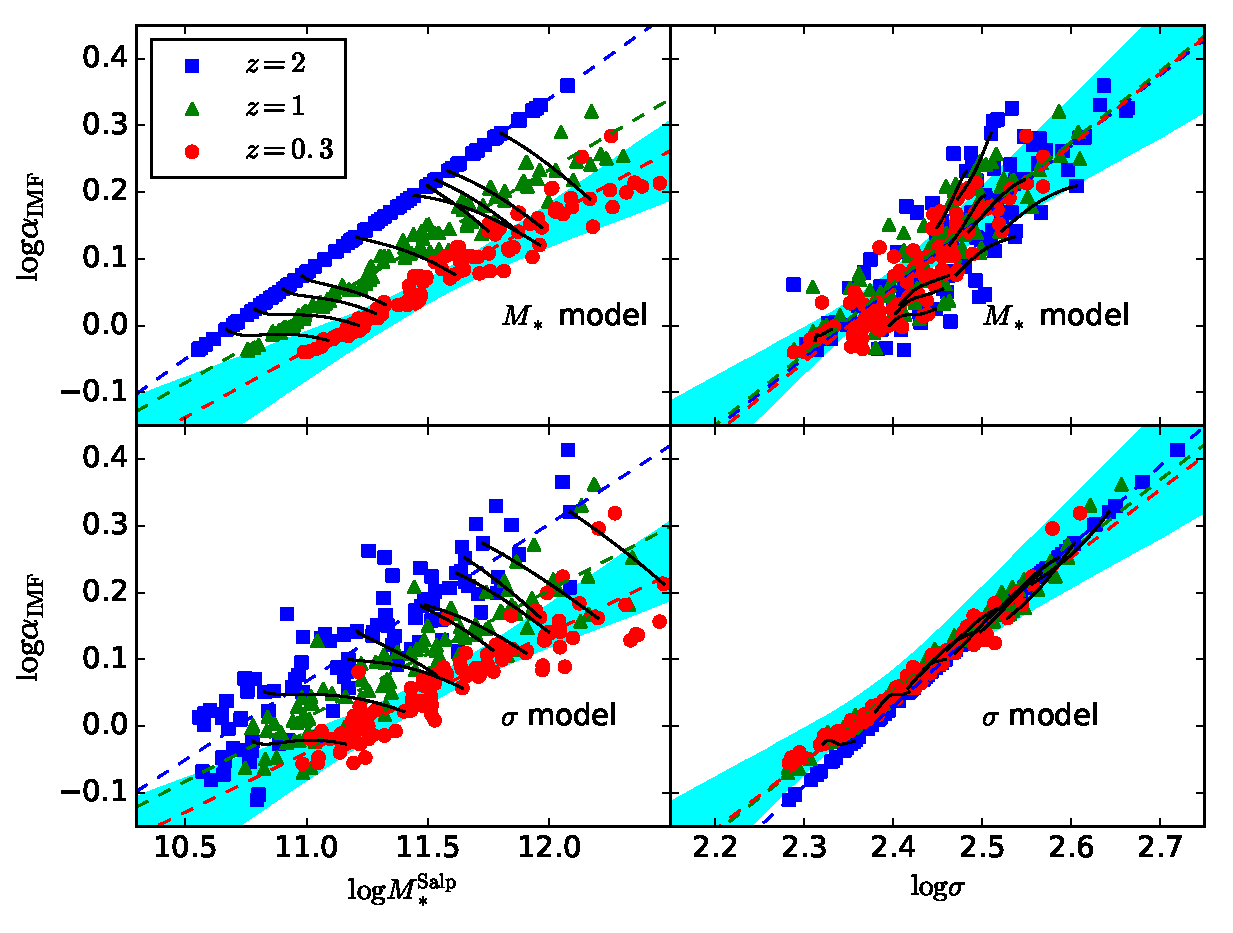
\includegraphics[width=\textwidth]{snapshots.eps}
 \caption{ IMF mismatch parameter $\aimf$ as a function of stellar mass ({\em left panels}) and central velocity dispersion ({\em right panels}) for the ``$M_*$ model'' ({\em top panels}) and ``$\sigma$ model'' ({\em bottom panels}) IMF recipes, at three different redshifts.
{\em Dashed lines:} Linear fit to the data in each redshift snapshot.
{\em Shaded regions:} Observational constraints from \citet{Son++15} ({\em left panels}) and \citet{Pos++15} ({\em right panels})
}
 \label{fig:snap}
\end{figure}
%
\begin{table}
 \caption{Best-fit parameters of \Eref{eq:mstarmodel} and \Eref{eq:sigmamodel} to the mock data shown in \Fref{fig:snap}. The third number in each set represents the residual scatter around the best fit relation.}
 \label{tab:oneparfit}
 \begin{tabular}{lcc}
 \hline
 Data set & Eq. \ref{eq:mstarmodel} fit & Eq. \ref{eq:sigmamodel} fit\\
 & $(a_*, b_*, s_*)$ & $(a_\sigma, b_\sigma, s_\sigma)$ \\
 \hline
% ``$M_*$ model'', $z=2$ & $(0.35, 0.07, 0.)$ & (2., -0.1, 0.1) \\
 ``$M_*$ model'', $z=2$ & (0.33, 0.07, 0.00) & (1.26, -0.09, 0.06) \\
``$M_*$ model'', $z=1$ & (0.26, 0.00, 0.02) & (1.03, -0.04, 0.06) \\
``$M_*$ model'', $z=0$ & (0.23, -0.06, 0.02) & (0.75, 0.00, 0.05) \\
``$\sigma$ model'', $z=2$ & (0.41, -0.04, 0.08) & (2.30, -0.35, 0.00) \\
``$\sigma$ model'', $z=1$ & (0.32, -0.12, 0.06) & (1.76, -0.24, 0.05) \\
``$\sigma$ model'', $z=0$ & (0.29, -0.20, 0.04) & (1.20, -0.15, 0.06) \\

 \hline
 \end{tabular}
\end{table}

As can be seen by comparing the left hand panels in \Fref{fig:snap} with the right hand panels, correlations between IMF and stellar mass correspond to similar correlations with velocity dispersion, and vice-versa. This is just a consequence of the tight correlation between galaxy stellar mass and velocity dispersion in the mock sample (and in observations). 
Trends of $\aimf$ with stellar mass and velocity dispersion, which we assumed in place at $z=2$, are mostly preserved by dry mergers down to $z=0$, but become less steep with time.

By $z=1$ a relatively large scatter is introduced in the $\aimf-\sigma$ space (right hand panels of \Fref{fig:snap}), even for the ``$\sigma$ model'' where the sample is initialized at $z=2$ with zero scatter. This is mostly driven by the evolution of galaxies in the most massive halos: these objects experience the highest merger rates and their change in velocity dispersion is correspondingly high. We will discuss this point more in the next Section.

For a given row in \Fref{fig:snap}, a look at the $z=2$ scatter plots in stellar mass and velocity dispersion space allows anyone to immediately identify which IMF recipe was used to produce the mock data.
The same procedure becomes nontrivial at $z=0$ due to scatter.
In order to test how accurately observations can discriminate between the two scenarios, we now perform fits in which the IMF can depend both on stellar mass and velocity dispersion:
\begin{equation}\label{eq:hybrid}
%\log{\aimf} = \frac{\partial \log{\aimf}}{\partial \log{M_*}}(\log{M_*} - 11) + \frac{\partial\log{\aimf}}{\partial\log{\sigma}}(\log{\sigma} - 2.3) + \log{\alpha_0}.
\log{\aimf} = a_*(\log{M_*} - 11) + a_\sigma(\log{\sigma} - 2.3) + b.
\end{equation}
In \Fref{fig:tracks} we plot the measured values of $a_*$ and $a_\sigma$ at each timestep.
In addition to the ``$M_*$ model'' and ``$\sigma$ model'' described above we also test a ``Hybrid model'' in which the IMF depends both on stellar mass and velocity dispersion as described by \Eref{eq:hybrid}, 
with $a_*=0.3$, $a_\sigma=1.5$, $b=0.0$.


%One of the goals of observational studies of the IMF in massive galaxies is to determine which, among the global properties of galaxies, is the fundamental quantity the IMF appears to depend on.

%Assuming that the IMF is fundamentally determined by one (or a small set of) global property of agalaxy, we would ideally like to observationally identify that 
%Ideally we would like to observationally determine which, among the global properties of galaxies, is the fundamental quantity the IMF depends on, if present at all
%Ideally, we would like to observationally determine what global quantity the IMF fundamentally depends on, if present at all



%\section{Discussion}\label{sect:discuss} 

%\subsection{Consistency checks}

%\subsection{Caveats}
%There's no scatter.
%We ignore progenitor bias.


\section{Conclusions}\label{sect:concl} 

\section*{acknowledgments}
%-------------------------------------------------------------------------------

%\acknowledgments

% Boilerplate:
%\input{acknowledgments2.tex}

%-------------------------------------------------------------------------------

\bibliographystyle{mnras}
\bibliography{references}
%-------------------------------------------------------------------------------


\end{document}

%===============================================================================
